\documentclass{beamer}

\usepackage[utf8x]{inputenc}

% Theme and options
% \usetheme{Madrid} % You can change this to another theme
% \usecolortheme{dolphin} % You can change this to another color theme

% Code formatting package
\usepackage{listings}
\usepackage{xcolor}
\usepackage{minted}
\usepackage{graphicx}
\usepackage{caption}
\usepackage{lipsum}
% \usepackage[backend=biber]{biblatex}
% \addbibresource{references.bib}


\newcommand\blfootnote[1]{%
  \begingroup
  \renewcommand\thefootnote{}\footnote{#1}%
  \addtocounter{footnote}{-1}%
  \endgroup
}

\mode<presentation>
{
  \usetheme[progressbar=foot,numbering=fraction,background=light]{metropolis} 
  \usecolortheme{default} % or try albatross, beaver, crane, ...
  \usefonttheme{default}  % or try serif, structurebold, ...
  \setbeamertemplate{navigation symbols}{}
  \setbeamertemplate{caption}[numbered]
} 

\title{Strength and Weaknesses of the C Programming Language}
\author{Danial Tariq}
\institute{Advanced Systems Programming}
\date{\today}

\begin{document}

\frame{\titlepage}

\begin{frame}[fragile]
    \frametitle{Strengths}

    \begin{columns}
        \begin{column}{0.5\textwidth}
            \begin{itemize}
                \item Control over layout of data structures down to individual bits.
                \item Manual memory management -- Makes it easier for developers to create more efficient memory allocation strategies.
                \item Highly portable -- pretty much every platform has a C compiler.
            \end{itemize}
        \end{column}
        \begin{column}{0.5\textwidth}
            \begin{minted}[frame=single,fontsize=\footnotesize]{c}
struct rtp_header {
uint16_t cc:4
uint16_t x:1;
uint16_t p:1;
uint16_t v:2;
uint16_t pt:7;
uint16_t m:1;
uint16_t seq;
uint32_t ts;
uint32_t ssrc;
}

char *buffer = malloc(BUFLEN);
// ...
                      \end{minted}
        \end{column}
    \end{columns}
\end{frame}
\begin{frame}[fragile]
    \frametitle{Weaknesses - Memory Safety}

    \begin{columns}
        \begin{column}{0.5\textwidth}
            
            \begin{itemize}
                \item Incredibly easy to introduce memory safety vulnerabilities.
                \item Lack of bounds checking -- this has been the cause of some of the most severe security vulnerabilities, e.g. Heartbleed, Crowdstrike outages.
                \item Lack of temporal safety -- use-after-free, double-free, etc.
            \end{itemize}

        \end{column}

        \begin{column}{0.5\textwidth}
            \begin{figure}
                \centering
                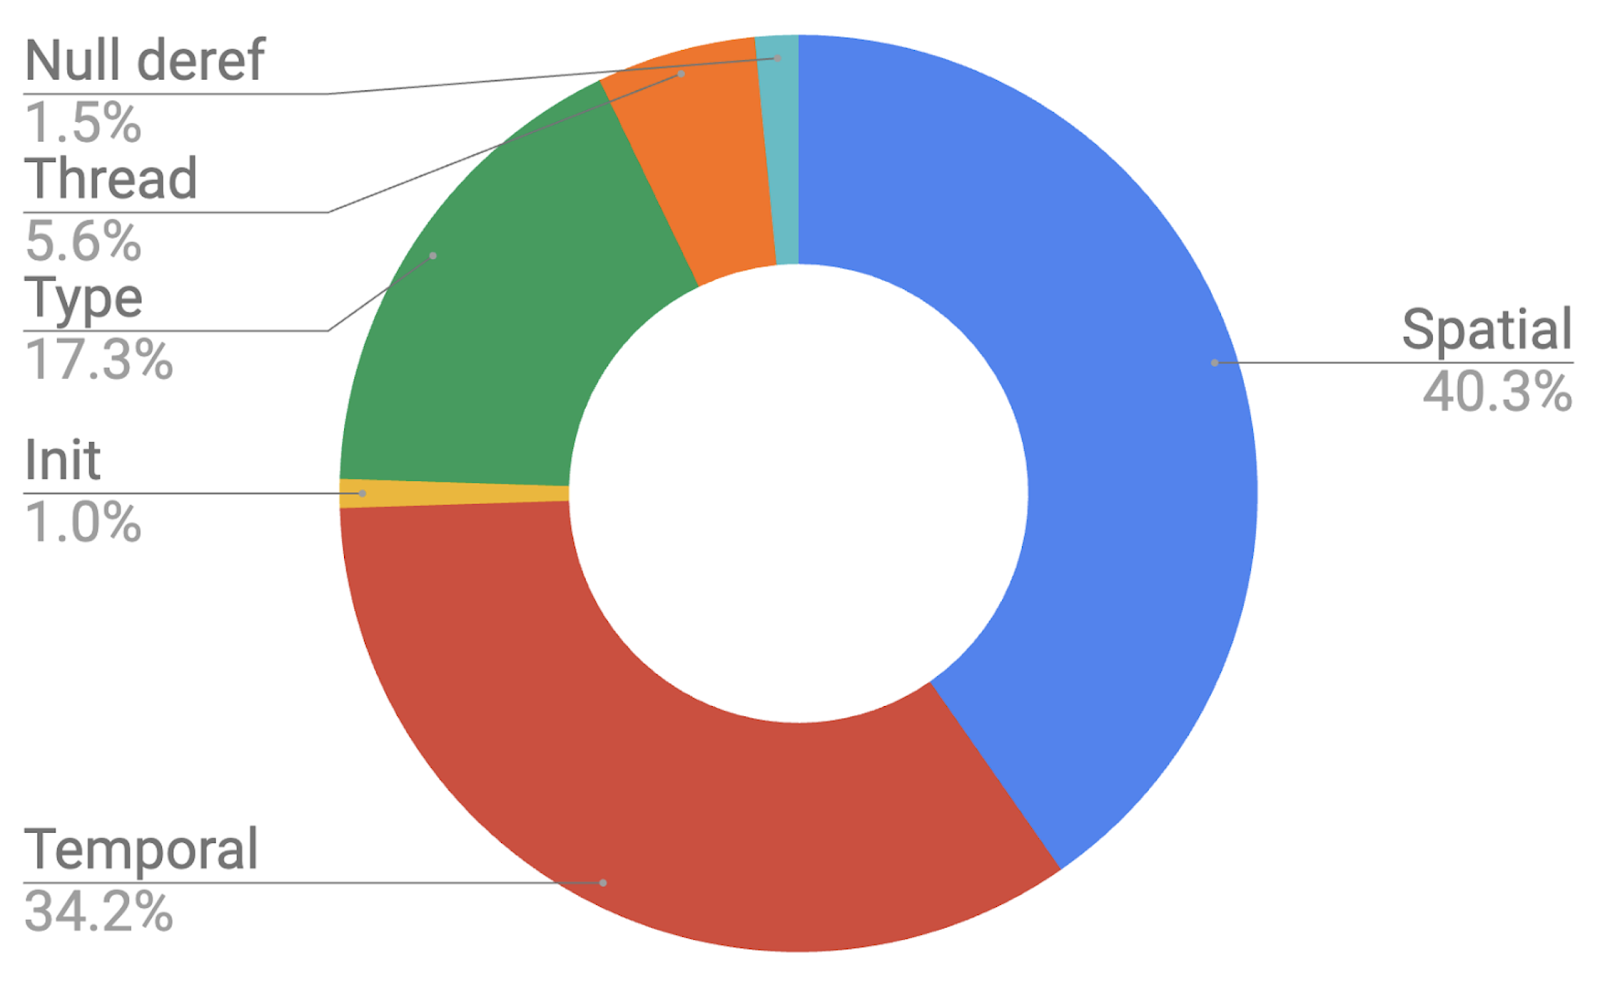
\includegraphics[width=1.0\textwidth]{google0-day.png}
                \caption*{Breakdown of memory safety zero-day exploits by vulnerability class}
            \end{figure}
        \end{column}
    \end{columns}
    \blfootnote{Source: Google Security Blog. \url{https://security.googleblog.com/2024/11/retrofitting-spatial-safety-to-hundreds.html}}
\end{frame}

\begin{frame}
    \frametitle{Weaknesses - Undefined Behavior}

    \begin{itemize}
        \item There are many cases where the C standard deliberately leaves the behavior of certain operations undefined.
        \item This is often done for performance reasons, but can lead to subtle bugs that are difficult to diagnose.
        \item This becomes even more challenging when you consider the behaviour of optimising compilers in the presence of undefined behaviour.
        \item This can also interfere with the programmer's mental model of the layout of data structures in memory.
    \end{itemize}
\end{frame}


% \begin{frame}
%     \frametitle{}

% \end{frame}

% % Slide 2: Example C Code
% \begin{frame}[fragile]
%     \frametitle{Example C Code}

%     Here is a simple C program that prints "Hello, World!" to the console:

% \begin{minted}{c}
% int main() {
%     printf("Hello, world!");
%     return 0;
% }
% \end{minted}
% \end{frame}



% \begin{frame}
%     \frametitle{Key Features of C}
%     \begin{itemize}
%         \item Simple and efficient \pause
%         \item Low-level access to memory
%         \item Rich set of operators
%         \item Functions for modular programming
%         \item Portability
%     \end{itemize}
% \end{frame}

% % Slide 4: Conclusion
% \begin{frame}
%     \frametitle{Conclusion}
%     \begin{itemize}
%         \item C is a powerful and widely-used programming language.
%         \item It forms the foundation for many other languages.
%         \item Learning C is valuable for understanding computer systems and programming fundamentals.
%     \end{itemize}
% \end{frame}

\end{document}
